\beginsong{Ye Jacobites}[
    wuw={Robert Burns, Musik aus Schottland},
    jahr={1791},
    pfiii={96}, 
    pfii={188}, 
    bo={436}, 
    kssiv={132}, siru={297},
]

\beginchorus
\endchorus
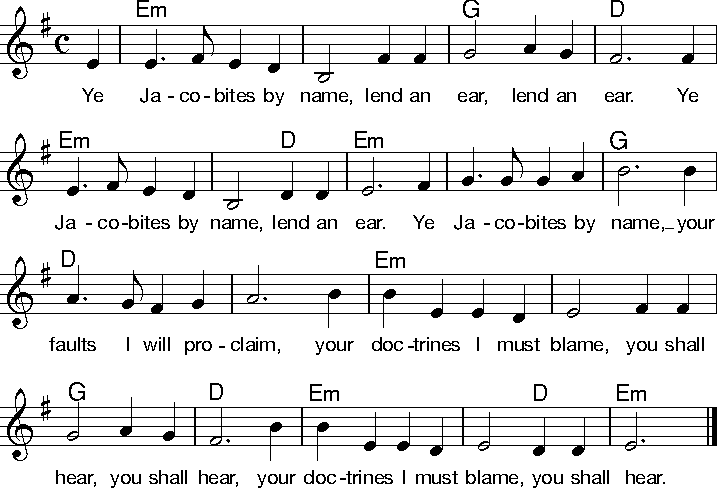
\includegraphics[draft=false, width=1\textwidth]{Noten/Lied103.pdf}	

\beginverse
What's \[Em]right and what is wrong, by the \[G]law, by the \[D]law?
what's \[Em]right and what is wrong, \[D]by the \[Em]law?
What's right and what is \[G]wrong, a \[D]short sword or a long,
a \[Em]weak arm or a strong, for to \[G]draw, for to \[D]draw,
a \[Em]weak arm or a strong, \[D]for to \[Em]draw.
\endverse

\newpage

\beginchorus
Ye ^Jacobites by name, lend an ^ear, lend an ^ear.
Ye ^Jacobites by name, ^lend an ^ear.
Ye Jacobites by ^name, your ^faults I will proclaim,
your ^doctrines I must blame, you shall ^hear, you shall ^hear,
your ^doctrines I must blame, ^you shall ^hear.
\endchorus

\beginverse
What ^makes heroic strife, famed a^far, famed a^far?
What ^makes heroic strife, ^famed a^far?
What makes heroic ^strife, to ^whet assassin's knife?
or ^haunt your parent's life with bloody ^war, bloody ^war,
or ^haunt your parent's life with ^bloody ^war.
\endverse

\printchorus

\beginverse
Then ^leave your schemes alone, in the ^state, in the ^state,
then ^leave your schemes alone, ^in the ^state.
Then leave you schemes a^lone, and a^dore the rising sun
and ^leave a man undone to his ^fate, to his ^fate,
and ^leave a man undone ^to his ^fate.
\endverse

\printchorus

\endsong

\beginscripture{}
Ein traditionelles schottisches Volkslied. Es richtet sich gegen die Jakobiten, Anhänger des 1688 vom englischen Parlament abgesetzten und aus England vertriebenen Stuartkönigs James II. Ziel der Jakobiten, die den Großteil des schottischen Adels in ihren Reihen hatten, war es, die Rückkehr James II. bzw. seiner Erbfolger zu ermöglichen. Dazu zettelten diese mehrere Aufstände (''Jacobite Risings'') an, von denen der letzte 1746 in der~ ''Schlacht bei Culloden'' niedergeschlagen wurde.
\endscripture
